\documentclass{standalone}
\usepackage{tikz}

\begin{document}
\usetikzlibrary{positioning,shapes,arrows,snakes}
\definecolor{yellowish}{HTML}{FFE699}
\definecolor{grayish}{HTML}{D9D9D9} 
\tikzset{
   rect/.style={
      align=center,
      text=black,    
      minimum width=2.5cm,
      minimum height=2cm}
}
\tikzset{
   done/.style={rect, fill=grayish }
}
\tikzset{
   todo/.style={rect, fill=yellowish}
}
\tikzset{
   arrow/.style={line width=1mm}
}
\centering

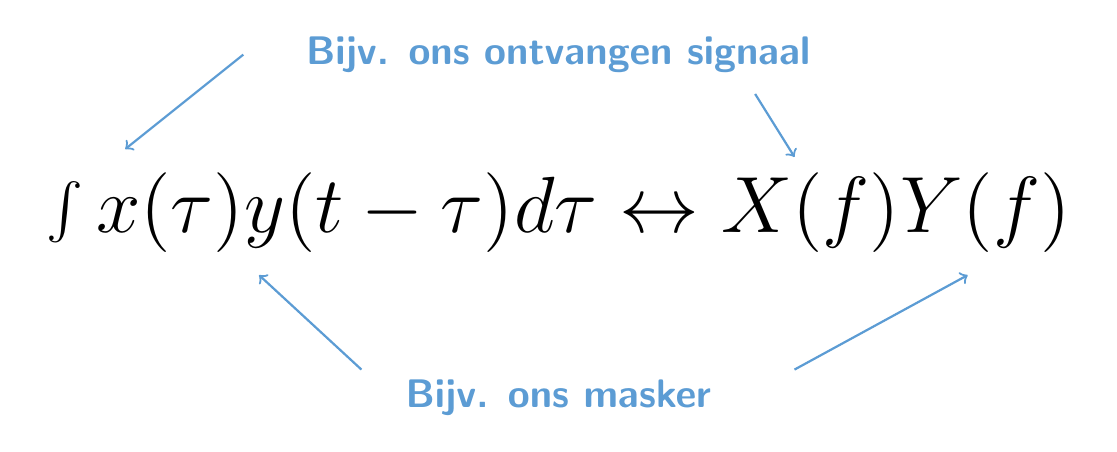
\begin{tikzpicture}[font=\Large\bfseries\sffamily]
   \definecolor{babyblueeyes}{rgb}{0.36, 0.61, 0.83}
   \draw (0,0) node[align=center,babyblueeyes]           {Bijv. ons ontvangen signaal};
   \draw (0,-4) node[below, align=center,babyblueeyes]   {Bijv. ons masker}; 
   \draw (0,-2) node[align=center,scale=2]{$\int x(\tau)y(t-\tau)d\tau \leftrightarrow X(f)Y(f)$};   
   \draw[->,babyblueeyes,thick] (-4,0) -- (-5.5,-1.2);
   \draw[->,babyblueeyes,thick] (2.5,-0.5) -- (3,-1.3);
   \draw[->,babyblueeyes,thick] (-2.5,-4) -- (-3.8,-2.8);
   \draw[->,babyblueeyes,thick] (3,-4) -- (5.2,-2.8);
\end{tikzpicture}
\end{document}